% Chapter 

\chapter{\color{thesisBlue} Using Generative models of naturalistic scenes to sample neural population tuning manifolds} % Main chapter title

\label{ch:maps} % For referencing the chapter elsewhere, use \ref{ch:maps} 

%----------------------------------------------------------------------------------------

% Define some commands to keep the formatting separated from the content 
%\newcommand{\keyword}[1]{\textbf{#1}}

%------------------------------------------------------------------------------------

\section{Introduction}
Research into sensory coding in the visual system focuses on determining what visual features neuronal activity covaries with, i.e. what information is it encoding. Traditional experiments looked at neural responses to simple stimuli such as small patches of light or oriented bars \parencite{Hubel1959}. These hallmark studies uncovered the simple/complex models of V1 neurons, which describe the way in which neurons integrate inputs from the \gls{lgn}. Orientation tuning of simple cells arises from overlapping ON-OFF regions of RGC inputs. Therefore, gabor stimuli are effective at driving neurons in early visual areas due to the precise arrangement of their inputs. Later in the visual hierarchy, such as V4, it becomes much more difficult to infer the exact tuning properties of neural inputs, and how they combine to form emergent tuning of these neurons. Neurons in area V4 only weakly respond to such stimuli as gabors, as they prefer complex combinations of many features such as contrast, color, orientation, curvature, etc \parencite{Sani2013,Tanigawa2010, Nandy2016}. It is not feasible to systematically test every combination of visual features to accurately describe feature tuning in such brain regions. Here we describe a method for efficiently exploring rich stimulus spaces to find relationships between sensory features and neural responses.

In these experiments, we used a \gls{gan} as our high-dimensional feature space. A \gls{gan} is a type of artificial neural network trained to represent the high-order statistics from a training set of data using a lower-dimensional set of `latent’ variables. In a \gls{gan} trained on faces for example, one of these variables is the age of the person \parencite{Karras2019}. The complex combinations of visual features that makes someone look older or younger actually represents a one-dimensional variable, and \glspl{gan} capture that. We sought to investigate if neurons in mid-level visual areas like V4 are tuned to the image statistics captured by this latent variable model. The problem is that the stimulus space is so large, it is impractical to just show random images and hope to find tuning. We developed a method to efficiently explore parts of the GANs latent space that are most likely to result in large neural responses from the population. 

While the idea of optimizing stimuli for neurons is not new, most of these studies focus on maximizing the response of single neurons \parencite{Ponce2019, Bashivan2019}.  It is unlikely that a single unique stimulus exists such that it maximally excites a diverse neural population. This is especially true in areas like V4, where neurons have complex tuning across many modalities \parencite{Pasupathy2002}. In fact, there are likely many unique stimuli that drive the neural population at similar levels due to contributions from different neurons. To contend with this difficulty, \gls{maps} efficiently searches the stimulus space by balancing optimization and exploration. Cowley et al (2017) demonstrated that optimizing for the $L^2$ norm of the population response vector results in a reasonable estimation of the response manifold \parencite{Cowley2017}. The goal of \gls{maps} isn't to optimize the stimuli for the neurons, but to maximize the amount of information gained from each stimulus presentation. This allows for a better description of the relationship between stimuli and neural tuning. A population of images "move" through the stimulus space by using kernel regression to estimate local gradients, and stepping along them. The images also morph to become more similar to other images that resulted in a better response from the population. By iterating through this process, we can collect a large amount of neural response data from unique stimuli in a relatively short amount of time. 


We used matrix electrode arrays (NeuroNexus, Ann Arbor, MI, USA) implanted in visual area V4 of rhesus macaques ({\it Macaca Mulatta}), to record population responses to GAN images. Over the course of a recording session, the animal passively viewed stimuli that were generated with our technique.

MAPS found a 20 dimensional stimulus subspace that was significantly linearly correlated with V4 neural activity. Our approach is more efficient than other currently accepted methods such as genetic algorithms, which get stuck showing the same images resulting in sub-optimal exploration of the stimulus and response spaces.

\section{Methods}

\subsection{Anesthetized Experiment}
The subject used in this study was one adult male rhesus macaque \textit{(Macacca Mulatta)}, Tw. All surgical and experimental procedures were performed in accordance with the National Institutes of Health \textit{Guide for the Care and Use of Laboratory Animals} \parencite{guide} and were approved by the University of Rochester Committee for Animal Research.

\subsubsection*{Surgical Procedures}
TW was given an initial dose of \textbf{$10 \frac{mg}{kg}$} ketamine i.m. to induce anesthesia. The animal was then maintained on \textbf{suftanil citrate (3– 6g/kg/h, i.v.), isoflurane ($0.5\%$), and nitrous oxide 1:2 in oxygen} throughout the experiment. We monitored ECG (electrocardiogram), temperature, expired $CO_2$, and \textbf{BLANK} in order to ensure depth of anesthesia. Craniotomies were made over V1 \textbf{(details: diameter, coordinates, etc.)} and V4 \textbf{(details: diameter, coordinates, etc.)} in the right hemisphere. The dura was reflected and then the craniotomies filled with \textbf{agaragar details}. Animals were then fit with contact lenses and paralyzed with \textbf{vencuronium bromide (0.2 mg/kg/h, i.v.)} before recording.

\subsubsection*{Neural Recordings}
Neurophysiological recordings were done using steriotactic implantation of Phase 3B neuropixels \parencite{Jun2017} connected to \textbf{amplifier details} before being recorded using SpikeGLX \textbf{spikeglx info}. Neuropixels were lowered normal to the surface of the cortex in V4 and allowed to baseline for around 30 minutes prior to recording. Following several sessions in V4, we recorded from V1 neurons 

\subsubsection*{Receptive Field Mapping}
Receptive fields were mapped by hand using \textbf{fancyFlashlight} on a whiteboard and listening for spikes. Stimuli were then sized to best cover the conglomerate receptive fields of simultaneously recorded neurons.

\subsubsection*{Visual Stimuli}
Naturalistic full-color images (as described in \ref{methods:gan}) were displayed on a gamma-calibrated 100Hz CRT monitor (ViewSonic, Brea, CA) placed 50-60cm from the animals' eyes. Stimulus control was done with ViSaGe system (Cambridge Research Systems, Rochester, UK) using crs 24-bit color mode in coordination with custom-written Matlab (Mathworks, Natick, MA; for optimization and display) and Python (GAN image generation) routines. Images were displayed on a grey background for 500ms with 1000ms inter-stimulus-intervals. 

\subsubsection*{Data Preprocessing: Anesthetized}
Spiking data was first run through Kilosort \parencite{Steinmetz2021} to extract individual neurons across channels. Neuron quality was then manually evaluated using Phy before being converted to NeuroData Without Borders (NWB) prior to further analyses.


\subsection{Alert Experiment}

\subsubsection*{Surgical Procedures}
Prior to any electrical recordings, the subject (Ro) was first implanted with a titanium head holder, trained on behavioral tasks, and then implanted with chronic electrode arrays. All surgeries we performed with isoflurane anesthesia, aseptic technique, and perioperative opiate analgesics in accordance with the National Institutes of Health \textit{Guide for the Care and Use of Laboratory Animals} \parencite{guide} and were approved by the University of Rochester Committee for Animal Research.

\subsubsection*{Head Holder Implantation} The subject was initially sedated with a 10mg/kg intramuscular injection of ketamine and administered with 0.25mg/kg midazolam, 0.011mg/kg glycopyrrolate, 25mg/kg cefazolin, and 0.2mg/kg meloxicam, all intramuscular. Once anesthetized, we intubated the animal with an endotrachial tube, shaved the animals head, inserted a catheter in the small saphenous vein for infusion of lactated Ringer's solution, then positioned the head in a stereotaxic frame. The anesthesia was maintained with 1.5\% isoflourane throughout the surgery. The surgical site was then thoroughly scrubbed with povidone iodine solution in the preparation of the sterile field. We made a horseshoe-shaped incision (6cm wide by 10cm anterior-posterior) using a \#10 scalpel blade starting from the right brow, cutting caudally parallel to the midline, and ending at the left brow. We then used bone curettes to retract the tissue and clear a large enough surface of skull for the head holder. Sterile gauze soaked in saline was used to keep the tissue moist throughout the surgery. The prefabricated titanium head holder (custum design machined by the university of Pittsburgh cite mat?) attaches to the skull using 16 6mm titanium screws (Veterinary Orthopedic Implants, Saint Augustine, FL) that go through 6 flange straps radially extending from the center of its base. We next bent the straps of the head holder so it fit tightly on the skull. We marked with pencil the final position of the head holder on the skull and made two small incisions in an x through the retracted tissue where the head holder would protrude. We then pushed the exterior portion of the head holder through the dermostomy in the retracted tissue and repositioned it back on the skull. We used a 2mm surgical drillbit and a custum drill stop set to the thickness of the skull to drill through the skull, starting with the lateral-most location of the head holder. Skrews were implanted one a time, alterniting across the midline, lateral to medial. Once each screw was implanted we used geristore (DenMat, Lompoc, CA, USA) to fill any gaps between the skull and head holder. After the geristor fully dried, we sutured the wound using a continuous running stitch to attach the subcutaneous fascia and simple interrupted stitches on top to fully connect the skin around the wound margin. Intramuscular injections of 25mg/kg cefazolin were administered every 12h for seven days post op, and 0.2mg/kg meloxicam every 24h for 3 days post op. The subject was allowed one month to recover before the start of training.

\subsubsection*{Behavioral Training} Prior to array implantation, the animal first underwent fixation training. The monkey sits 50cm away from a 120Hz ViewPixx/3D monitor (VPixx Technologies, Saint-Bruno, QC, Canada). We used Matlab (The MathWorks, Inc) and Psychtoolbox to control the experiments and present visual stimuli. Eye position was tracked with an Eyelink 1000 IR eye tracking camera (SR Research, Ottawa, Ontario, Canada), and the monkey was given water reward for fixating on a central dot. Once the monkey understood the basic reward contingencies he was implanted with two 128 channel matrix electrode arrays (NeuroNexus, Ann Arbor, MI, USA).

\subsubsection*{Array Implantation} The monkey was given intramuscular injections of ketamine, medazolam, glycopyrrolate, cefazolin, and meloxicam at the same doses described earlier for the headpost holder surgery. Similarly, the monkey was intubated, shaved, catheterized, and positioned in the stereotactic frame in the same manner. Again the animal was maintained on 1.5\% anesthesia throughout the surgery. We marked the stereotactic coordinates for prefrontal cortex (30mm anterior, 21mm lateral, 25mm dorsal) and visual area V4 (0mm anterior, 0mm lateral, 27mm dorsal) as well as estimated locations for the two array pedestals (NeuroNexus, Ann Arbor, MI, USA) prior to making the incision. Once we planned out the location of the pedestals and craniotomies we made the incision with a size 10 scalpel blade, starting on the posterior surface of the cranium. The incision was made just off the midline (away from the hemisphere we implanted in) and continued until about 1cm away from the margin around the head holder, leaving room to ensure that enough healthy tissue remained between the incision and head holder. We then cut a hemicircle around the head holder, again leaving enough healthy tissue to be able to suture the wound and continued just off the midline up to the brow. The final incision started halfway through the hemicircular incision, perpendicular to the midline, and continued 10cm laterally. We used bone curettes to retract the tissue while minimizing muscle damage, and again kept the retracted tissue hydrated with sterile gauze and saline. Once the skull was sufficiently cleaned, we marked the location of the craniotomies in pencil using stereotactic coordinates. The pedestals were both placed on the midline, one anterior to the head holder (PFC), and the other posterior to the head holder (V4). Similar to the head holder surgery, we then bent the legs of the two pedestals to fit tightly onto the skull and marked the location of each screw with a pencil. The animal was then administered a second intramuscular dose of cefazolin. We used 8 and 10 6mm titanium screws (Veterinary Orthopedic Implants, Saint Augustine, FL) for the PFC and V4 pedestals respectively. After the pedestals were secured we used a 19mm diameter trephine to do the PFC craniotomy followed by kerrison punches to remove any pieces of bone around the perimeter. The animal was then administered a 0.5mg/kg intramuscular dose of dexmethasone. Afterward, we used a drimmel to smooth down a trench going from the pedestal to the craniotomy in order to prevent the wire bundle from snagging or bending. We next cut the dura on three sides of a 1cm square and retracted it. A 128 channel matrix electrode array (NeuroNexus, Ann Arbor, MI, USA) was inserted dorsal to the principal sulcus, using a microdriver (Zaber, Vancouver, British Columbia, Canada) attached to an all-angle manipulator (NeuroNexus, Ann Arbor, MI, USA). Once the array was in place, we inserted the reference wire under the dura, sutured it closed with nurolon sutures (5-0 dissolving sutures), and covered the craniotomy with duragen (Integra Life Sciences co.). The animal was injected with Buprinex SR IM every two hours, starting 6 hours into the surgery until we finished. We then used two titanium plates to cover and protect the craniotomy by screwing them into the skull in the same manner as the pedestals and headpost. After the craniotomy was secure we covered the trench and wire bundle with kwik-sil and filled any gaps under the PFC pedestal with geristore. We then sutured around the anterior wound margin back to the lateral incision using the same procedure as the head holder sutures. These same steps from craniotomy to suturing were replicated for the implantation of the V4 array. Post operative care included administration of 25mg/kg cefazolin every 12h for seven days, and 0.2mg/kg meloxicam every 24h for 3 days.

\susubsection*{Data Preprocessing: Alert.}
A initial automatic step of maximum likelihood estimation of gaussian distribution parameters. After this automatic step, results were manually refined using custom routines for MatLab \parencite{Kelly2007}


\subsection{Data Analysis}
All analyses were done with custom routines for Matlab 2022b (The MathWorks, Inc). Due to limitations in real-time spike sorting, a simplified definition of neural response was used during optimization. During the experiment, a neuron's response was defined as the number of threshold crossings (-4 standard deviations below the median noise) that occurred in a 500ms window from stimulus onset. 


\subsection*{Generative Adversarial Network}
\label{methods:gan}
\glsreset{gan}
\Glspl{gan} are a type of artificial neural network that learn low-dimensional representations of higher-dimensional data, such as images \cite{Karras2019}. \glspl{gan} trained to generate images learned to map high-order image statistics onto a set of lower-dimensional latent variables. The \gls{gan} used in these experiments had a 128-dimensional input (latent) space, and was trained on the Cifar-10 image data set as described previously \cite{Fruend2018}. 

\subsection{Particle Swarm}
Particle swarm utilizes a hive-mind approach to solve optimization problems. Each `particle’ corresponds to a point in the high dimensional stimulus space (an image), and travels through the space in order to maximize the $L^2$ norm of the population response. By moving through the stimulus space, the images change along latent feature dimensions, resulting in smooth image manipulation. Particles move through the stimulus space by integrating information about local gradients and neural responses to other particles. Particles therefore both compete and collaborate in order to explore the stimulus and response spaces. \\
\gls{maps} is initialized with three generations of random points for each of 64 particles. This gives the kernel regression a history to estimate gradients. For subsequent generations, each particle takes a step $S_p$ according to three terms: the estimated local gradient $\nabla e_p$,  the weighted sum of vectors towards particles that resulted in better neural responses $G_p$, and a momentum term $M_p$ (Equation 1).
\begin{equation}
	S_p= c_1 r_{1p} \nabla e_p+ c_2  r_{2p} G_p+b M_p
\end{equation}

The constants $c_1$ and $c_2$ are learning rates for the gradient and global information components respectively, while $b \in [0,1]$ is a decay term for the momentum. The stochastic scaling factors $r_{1p}$ and $r_{2p} \sim U(0,1)$ help circumvent the problem of choosing a correct step size. Too large and particles will jump over maxima, but too small and it will take too long to converge, so step sizes are pulled from a uniform distribution for each particle each generation.

We used kernel regression to estimate the gradient according to each particles’ personal history. This way, each particle travels along its' local gradient, independent of how each other particle moves. 

\begin{equation}
	\nabla e_p (x^* )=\frac{1}{t-1} \sum_{k=1}^{t-1} \nabla w_k (x^* )  A_k
\end{equation}

\begin{equation}
	\nabla w_k (x^* )=\frac{2K(x^*,x_k) \sum_{l=1}^{t-1} (x_k-x_l)K(x^*,x_l)} {h^2\left(\sum_{l=1}^{t-1}K(x^*, x_l)\right)^2}
\end{equation}

where

\begin{equation}
	A_k = \sum_{j=1}^{t-1}||r_k||+||r_k-r_j||
\end{equation}

and

\begin{equation}
	K(x,y)=e^{- \frac{||x-y||}{h^2}}
\end{equation}

The next component (Equation \ref{globalPart}) is a weighted sum that uses information about the global response manifold to predict where good parts of the space is. Stimuli that resulted in a large neural response from many neurons pull the particle density toward them. Again, $x_p$ and $r_p$ represent the stimulus embedding vector and the neural response vector respectively for particle $p$. $G_p$ is the sum of unit vectors towards all the points which resulted in better neural responses $x_k, k = 1,...,u$, weighted by how much better that response $r_k, k = 1,...,u$ was than the current point $r_p$.

\begin{equation}
	%G_p = ||\sum_{k=1}^{u}(||r_k||-||r_p||) ||\label{globalPart}
	G_p = \sum_{k=1}^{u}\frac{(||r_k||-||r_p||)}{\sum_{j=1}^{u}||r_j||-||r_p||} \frac {x_k-x_p}{||x_k-x_p||}\label{globalPart}
\end{equation}

\subsection{Genetic Algorithm}


\section{Results}
We tested our algorithm in two stimulus spaces, the latent space of a generative adversarial net and a gabor pyramid of equal dimensionality, and compared it's performance against a genetic algorithm in the same spaces. This allows us to demonstrate two key findings, that our method is flexible to the stimulus space used, and outperforms other state of the art approaches. 


\begin{figure}
	\centering
	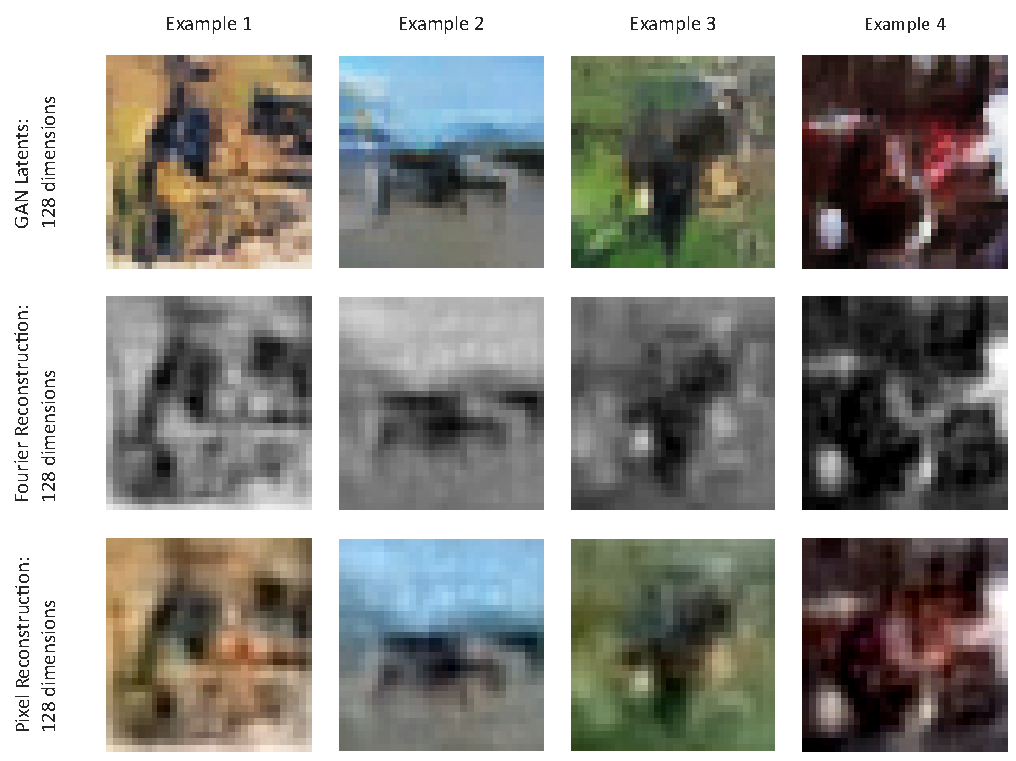
\includegraphics[width=172mm]{exampleImagesWreconstruction.pdf}
	\caption{Caption}
	\label{fig:exampleReconstructions}
\end{figure}

\begin{figure}
	\centering
	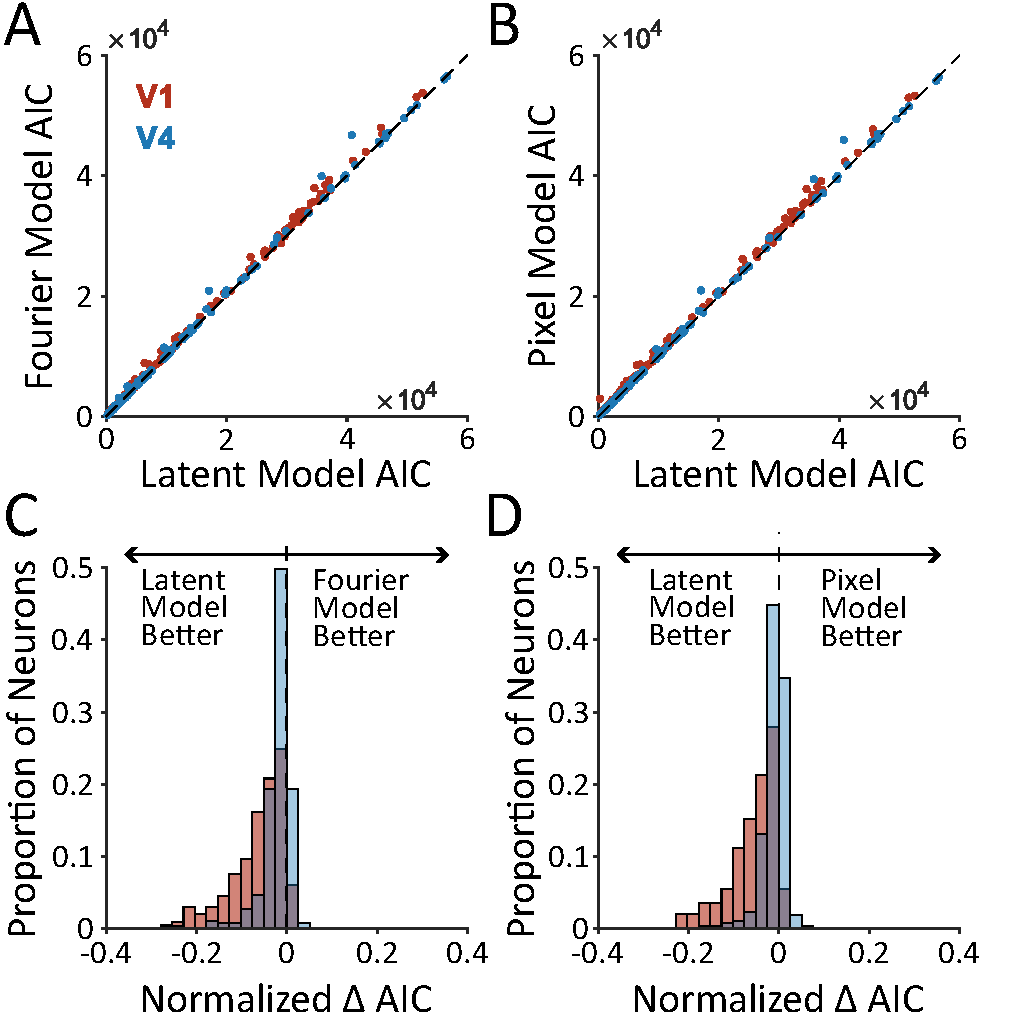
\includegraphics[width=86mm]{LatentVsFourierVsPixelModels.pdf}
	\caption{Caption}
	\label{fig:modelAICs}
\end{figure}


\section{Discussion}


NOTES: \\
Rates are high because we cant spike sort on the fly so units are most likely multi-unit.\\
To set this paper apart we need to emphasize that this is NOT about optimizing the stimulus for neurons but using optimization as an exploratory tactic \\
(about genetic algorithm)The persistence of certain individuals within the population result in the same point in latent space being shown multiple times, which is antithesis to our goal of exploring the relationship\\

\section{Conclusion}

%------------------------------------------------------------------------------------



%------------------------------------------------------------------------------------


 